\section{Representations of quadratics}
Consider the quadratic equation $ax^2+bx+c=0$ (and/or its graph, $y=ax^2+bx+c$). Given the quadratic in this form, and assuming that $a=1$ and also that the quadratic will factorise (these things are assumed throughout this section), we can find other useful information about (or if you want to think about it this way, forms of) this quadratic.

\subsection{Y-intercept}
The point at which the quadratic's graph crosses the y-axis, or rather, its coordinate when $x=0$. It is $c$ from $y=ax^2+bx+c$, because when $x=0$, $ax^2+bx$ must also equal $0$.
\begin{IEEEeqnarray}{sL}
    Equation: & y=x^2+2x-24
    \nonumber \\
    Y-intercept: & (0, -24)
\end{IEEEeqnarray}

\subsection{Factorisation}
A factorised version of the quadratic in the form $(x+m)(x+n)$. Useful for finding the roots. For $y=ax^2+bx+c$, $m$ and $n$ are two numbers that sum to $a$ and multiply to $b$.
\begin{IEEEeqnarray}{sL}
    Equation: & y=x^2+2x-24
    \nonumber \\
    Factorisation: & (x+6)(x-4)
\end{IEEEeqnarray}

\subsection{Roots}
The roots (or solutions) are the values of $x$ that satisfy $ax^2+bx+c=0$. They are also the x-coordinates at which $y=ax^2+bx+c$ crosses the x-axis. To find them, take $m$ and $n$ from the quadratic's factorisation, and multiply by $-1$.
\begin{IEEEeqnarray}{sL}
    Factorisation: & (x+6)(x-4)
    \nonumber \\
    Roots: & x=-6 \textrm{ or } x=4
\end{IEEEeqnarray}

\subsection{Completed the square}
This version takes the from $(x+p)^2+q$. It's useful for finding the turning points of the graph. For $y=ax^2+bx+c$, $p=\frac{b}{2}$, and $q=c-q^2$.
\begin{IEEEeqnarray}{sL}
    Equation: & y=x^2+2x-24
    \nonumber \\
    Completed the square: & (x+1)^2-25
\end{IEEEeqnarray}

\subsection{Turning point}
The turning point of the graph, found using the completed the square form of the equation. The x-coordinate is $-p$, because this would make the entire expression as small as possible ($0$, because no square term can be smaller), and the y-coordinate is simply $q$, because that will be all that's left when $(x+p)^2=0$.
\begin{IEEEeqnarray}{sL}
    Completed the square: & (x+1)^2-25
    \nonumber \\
    Turning point: & (-1, -25)
\end{IEEEeqnarray}

\subsection{Sketch}
Sketches of the graph should have their intercepts labelled, as well as the turning point.

So for $y=x^2+4x+3$ (the other one was too big to draw nicely):

\adjustbox{margin=1cm}{
    \pgfplotsset{ticks=none}
    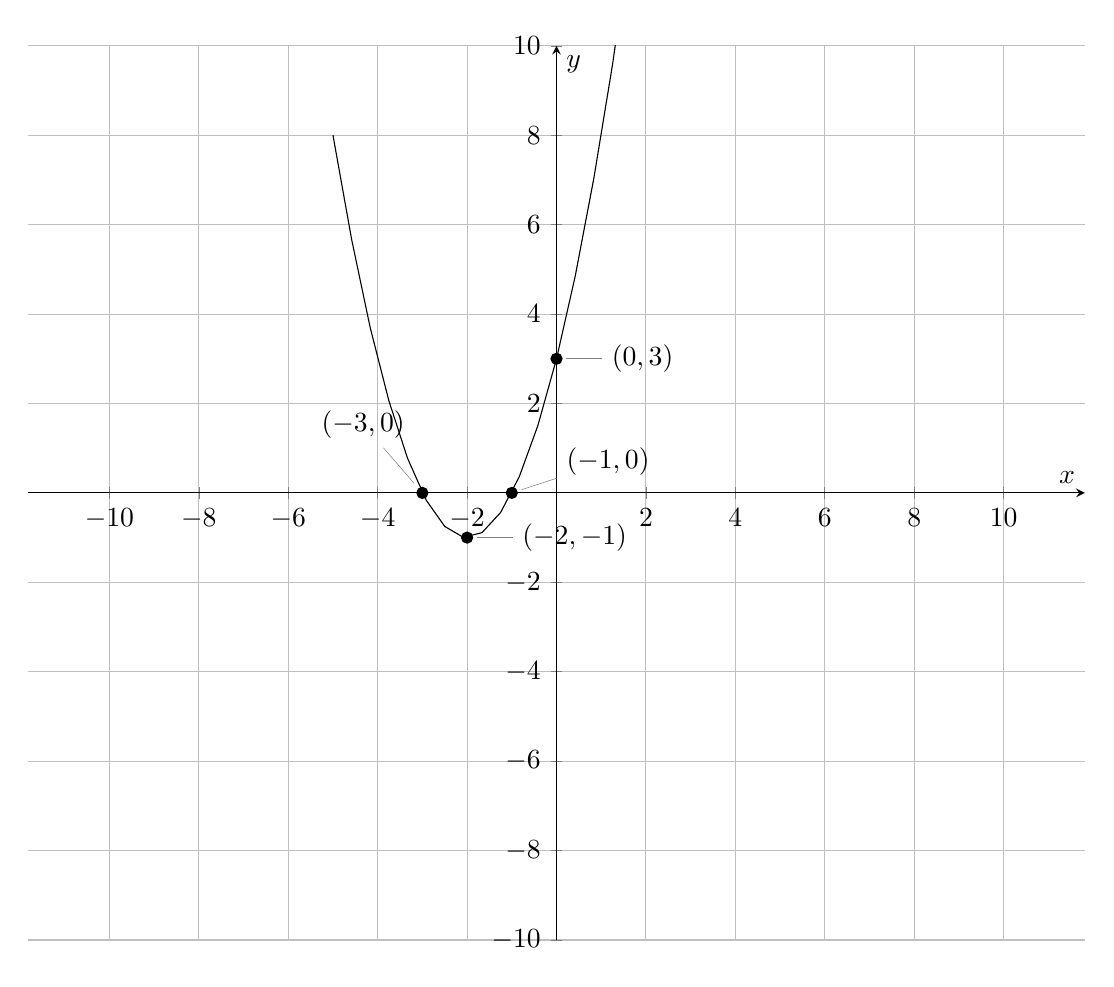
\begin{tikzpicture}[baseline]
        \begin{axis}[
            axis y line=center,
            axis x line=middle,
            axis equal,
            grid=both,
            xmax=10,xmin=-10,
            ymin=-10,ymax=10,
            xlabel=$x$,ylabel=$y$,
            width=15cm,
            anchor=center,
            ]
            \addplot[mark=none] {x^2+4*x+3};
            \addplot[mark=*] coordinates {(-2,-1)} node[pin=right:{$(-2, -1)$}]{} ;
            \addplot[mark=*] coordinates {(-3,0)} node[pin=100:{$(-3, 0)$}]{} ;
            \addplot[mark=*] coordinates {(-1,0)} node[pin=10:{$(-1, 0)$}]{} ;
            \addplot[mark=*] coordinates {(0,3)} node[pin=right:{$(0, 3)$}]{} ;
        \end{axis}
    \end{tikzpicture}
}

\section{Properties of quadratics}
There are certain key properties of quadratics in the form $ax^2+bx+c$.

\subsection{Factorising with integers}
This means that the quadratic can be factorised into the form $(ax+b)(cx+d)$ where $a$, $b$, $c$, and $d$ are all integers. Only some quadratics have this property. You can find out whether a quadratic has an integer factorisation by putting it into the quadratic formula $\frac{-b\pm\sqrt{b^2-4ac}}{2a}$. If the discriminant (the part under the square root) is a square number, then the quadratic can be factorised with integers, otherwise it cannot.

\subsection{Two x-intercepts}
This means that the quadratic's graph crosses the x-axis at 2 points, and therefore means that there are 2 different solutions to the equation when the quadratic is set equal to 0.

\subsection{Repeated x-intercept}
This means that the quadratic's graph touches the x-axis at only one point. If the quadratic factorised, it would be in the form $(ax+b)^2$. Setting the quadratic equal to 0 would only yield one solution.

\subsection{No x-intercepts}
This means that the quadratic's graph stays above or below the x-axis at all times, never touching it at any point. Any quadratics that have this property definitely will not factorise with integers, as this would imply it having either one or two x-intercepts. In fact, when set equal to 0, these quadratics have no real solutions.

\subsection{Has a minimum point}
This means that the quadratic's graph is `happy' (looks like a smiley face, with the turning point as the lowest point in the graph, and the graph extending infinitely upwards). Quadratics in the form $ax^2+bx+c$ where $a>0$ have this property.

\subsection{Has a maximum point}
This means that the quadratic's graph is `unhappy' (looks like an upside-down smiley face, with the turning point as the highest point in the graph, and the graph extending infinitely downwards). Quadratics in the form $ax^2+bx+c$ where $a<0$ have this property.

\subsection{Y-intercept}
The point at which the quadratic's graph crosses the y-axis. Equal to $c$ for quadratics in the form $ax^2+bx+c$.

\section{Quadratics in disguise}
Some quadratics may be disguised. For example, if there are other indices involved before the term gets squared. For example:
\begin{IEEEeqnarray}{rCl?s}
    x^4 + x^2 + 4 & = & 0 & // can be rewritten as
    \nonumber \\
    (x^2)^2 + (x^2) + 4 & = & 0 & // let $y = x^2$
    \nonumber \\
    y^2 + y + 4 & = & 0 & // and solve normally
\end{IEEEeqnarray}
Don't forget, after solving for $y$, to then sub $x^2$ back in and solve for $x$ 

This can also happen with fractions ($x^{\frac{2}{3}}+x^{\frac{1}{3}}+3$), or addition when $x$ is used in the exponent ($4^{2x}+4^{x+1}+6$). In each case, find something to substitute so that you're left with a term squared, followed by that same linear term, followed by constant. Then it should be fine to solve, for the substituted variable, substitute $x$ back in, and solve for $x$.